% NOTE: This draft uses IEEEtran so it compiles today. Before submission to IEEE Access, switch to
% the official IEEEaccess.cls from the IEEE Author Center and paste the content in.
\documentclass[journal]{IEEEtran}

\usepackage{graphicx}
\usepackage{tikz}
\usetikzlibrary{positioning,arrows.meta}
\usepackage{amsmath}
\usepackage{url}

\newcommand{\todo}[1]{\textbf{[TODO: #1]}}
% AUTO-GENERATED from repo data — DO NOT hand-edit numbers. Regenerate: node scripts (see papers/README).
% Every macro = a real measured value from the cited source file.

% ---- per-subject 5-fold CV mean accuracy (percent) ----
\newcommand{\AccOne}{86.7}% source: tests/fixtures/S001/cv_accuracy.json
\newcommand{\AccTwo}{86.7}% source: tests/fixtures/S002/cv_accuracy.json
\newcommand{\AccThree}{60.0}% source: tests/fixtures/S003/cv_accuracy.json
\newcommand{\AccFour}{68.9}% source: tests/fixtures/S004/cv_accuracy.json
\newcommand{\AccFive}{57.8}% source: tests/fixtures/S005/cv_accuracy.json
\newcommand{\AccSix}{33.3}% source: tests/fixtures/S006/cv_accuracy.json
\newcommand{\AccSeven}{93.3}% source: tests/fixtures/S007/cv_accuracy.json
\newcommand{\AccEight}{66.7}% source: tests/fixtures/S008/cv_accuracy.json
\newcommand{\AccNine}{35.6}% source: tests/fixtures/S009/cv_accuracy.json
\newcommand{\AccTen}{57.8}% source: tests/fixtures/S010/cv_accuracy.json
\newcommand{\AccMin}{33.3}% source: min over tests/fixtures/*/cv_accuracy.json
\newcommand{\AccMax}{93.3}% source: max over tests/fixtures/*/cv_accuracy.json

% ---- browser-vs-MNE agreement (machine precision) ----
\newcommand{\FilterR}{1.0}% source: tests/pipeline/multisubject.test.ts (filterR, 12 dp)
\newcommand{\CspFrobMin}{\ensuremath{6.6\times10^{-15}}}% source: multisubject test (CSP Frobenius)
\newcommand{\CspFrobMax}{\ensuremath{1.7\times10^{-14}}}% source: multisubject test (CSP Frobenius)
\newcommand{\LdaDiffMin}{\ensuremath{1.7\times10^{-13}}}% source: multisubject test (LDA weight diff)
\newcommand{\LdaDiffMax}{\ensuremath{2.4\times10^{-12}}}% source: multisubject test (LDA weight diff)

% ---- dataset / counts ----
\newcommand{\Nsubjects}{10}% source: tests/fixtures/subjects.json
\newcommand{\Nskipped}{0}% source: tests/fixtures/subjects.json
\newcommand{\Nepochs}{45}% source: tests/fixtures/*/params.json n_epochs
\newcommand{\Nchannels}{64}% source: params.json n_channels
\newcommand{\Fs}{160}% source: params.json fs_hz
\newcommand{\Ntimes}{321}% source: params.json epoch.n_times
\newcommand{\Ntests}{40}% source: npx vitest run (Test Files 13 / Tests 40)

% ---- method constants (match the code/oracle exactly) ----
\newcommand{\FirLo}{8}% source: params.json filter.cutoff_hz
\newcommand{\FirHi}{30}% source: params.json filter.cutoff_hz
\newcommand{\FirTaps}{165}% source: params.json filter.numtaps
\newcommand{\Tmin}{0.5}% source: params.json epoch.tmin_s
\newcommand{\Tmax}{2.5}% source: params.json epoch.tmax_s
\newcommand{\CspReg}{0.1}% source: params.json csp.reg
\newcommand{\CspComp}{4}% source: params.json csp.n_components
\newcommand{\LdaShrink}{0.1}% source: params.json lda.shrinkage
\newcommand{\Folds}{5}% source: params.json cv.n_splits
\newcommand{\Seed}{42}% source: params.json cv.random_state

% ---- oracle environment ----
\newcommand{\MneVer}{1.8.0}% source: subjects.json env
\newcommand{\SklearnVer}{1.5.2}% source: subjects.json env
\newcommand{\ScipyVer}{1.14.1}% source: subjects.json env
\newcommand{\NumpyVer}{2.0.2}% source: subjects.json env
\newcommand{\PyVer}{3.12.12}% source: subjects.json env

% ---- benchmark (real, reference run) ----
\newcommand{\WorkerOneX}{1696}% source: benchmarks/results.json conditionsWorker 1x
\newcommand{\WorkerOneXStd}{20}% source: benchmarks/results.json conditionsWorker 1x
\newcommand{\ProxyOneX}{1013}% source: benchmarks/results.json conditionsMain 1x
\newcommand{\ProxyFourX}{3954}% source: benchmarks/results.json conditionsMain 4x
\newcommand{\ProxySixX}{5992}% source: benchmarks/results.json conditionsMain 6x
\newcommand{\PeakHeap}{192.2}% source: benchmarks/results.json memory.peakMB
\newcommand{\BaseHeap}{9.0}% source: benchmarks/results.json memory.baseMB
\newcommand{\CrossLo}{1723}% source: benchmarks/results.json crossSubject
\newcommand{\CrossHi}{1763}% source: benchmarks/results.json crossSubject
\newcommand{\Nreps}{12}% source: benchmarks/results.json method
\newcommand{\HwCpu}{Apple M4}% source: benchmarks/results.json hardware
\newcommand{\HwCores}{10}% source: benchmarks/results.json hardware
\newcommand{\HwRam}{17.2}% source: benchmarks/results.json hardware (GB)
\newcommand{\HwBrowser}{Chromium 148.0.7778.96}% source: benchmarks/results.json hardware


\begin{document}

\title{A Validated, Fully Client-Side EEG Motor-Imagery Analysis Tool:\\
Machine-Precision Equivalence to MNE-Python in the Browser}

\author{Eugene~Cha%
\thanks{Eugene Cha is with \todo{affiliation} (e-mail: \todo{email}).}%
\thanks{ORCID: \todo{author ORCID}.}}

\markboth{Preprint draft --- IEEE Access submission to use IEEEaccess.cls}{Cha: Client-Side EEG Analysis}

\maketitle

\begin{abstract}
Reproducing electroencephalography (EEG) motor-imagery analyses typically requires installing a
native Python scientific stack, which is a barrier for students, clinicians, reviewers, and users of
restricted or low-specification hardware. We present an open-source tool that runs a complete
motor-imagery pipeline---bandpass filtering, epoching, Common Spatial Patterns (CSP), and Linear
Discriminant Analysis (LDA) with cross-validation---entirely in a web browser, with no backend and
no installation, performing the heavy computation in a Web Worker. To guard against silent numerical
drift when re-implementing a scientific pipeline in a new language, we treat MNE-Python and
scikit-learn as a reference oracle and validate each stage against dumped fixtures. Across all
\Nsubjects{} tested subjects of the PhysioNet EEG Motor Movement/Imagery Database, the browser
pipeline reproduces the reference to machine precision: filter Pearson $r=\FilterR$, CSP
projection-matrix Frobenius differences between \CspFrobMin{} and \CspFrobMax{}, LDA weight
differences between \LdaDiffMin{} and \LdaDiffMax{}, and identical cross-validation accuracies. We
report real in-browser runtime and memory measurements. The contribution is a validated client-side
reproduction with a multi-subject equivalence study and an accessibility argument, not a new
algorithm.
\end{abstract}

\begin{IEEEkeywords}
Electroencephalography, brain-computer interfaces, common spatial patterns, reproducibility,
client-side computing, web technologies, edge computing.
\end{IEEEkeywords}

\section{Introduction}
\IEEEPARstart{M}{otor-imagery} BCIs decode imagined movement from EEG and are widely used in
research and teaching. The standard analysis---spatial filtering, CSP feature extraction, and a
linear classifier---is well established, but \emph{running} it usually means installing MNE-Python
and a native dependency chain~\cite{gramfort2013mne}. That installation cost is a practical barrier
to reproducibility and to use on managed, shared, or low-specification machines. We ask whether the
same analysis can run, unchanged in result, with nothing more than a web browser, and whether such a
re-implementation can be \emph{proven} equivalent to the reference library. Our contributions are:
(i) a fully client-side, install-free EEG motor-imagery pipeline that performs heavy computation off
the main thread in a Web Worker; (ii) a validation methodology that establishes machine-precision
equivalence to an MNE-Python/scikit-learn oracle, demonstrated across \Nsubjects{} subjects; and
(iii) real in-browser performance measurements supporting an accessibility argument. We claim no new
algorithm.

\section{Related Work}
We position the work against two categories. \emph{Reproducible Python pipelines} build on
MNE-Python and therefore require installation~\cite{mnebidspipeline,meggie,eegpipeline,pylossless,eegpype};
they are powerful but not install-free, and not designed to run from a link in a browser.
\emph{Browser and low-cost-hardware BCI tools} emphasize live acquisition or
education~\cite{webbci,bci2000web,neuroblock,pieeg}; to our knowledge they do not establish numerical
equivalence of an offline analysis pipeline to a reference library. The gap we target---an
install-free analysis tool with \emph{validated} equivalence to MNE-Python---appears unoccupied to
our knowledge~\todo{complete literature sweep to confirm the gap and add citations}.

\section{Methods}
\subsection{Data}
We use the PhysioNet EEG Motor Movement/Imagery Database~\cite{schalk2004bci2000,goldberger2000physionet}:
imagery runs R04/R08/R12 (left- vs.\ right-hand imagery), \Nchannels{} channels at \Fs~Hz, yielding
\Nepochs{} epochs per subject after event extraction.

\subsection{Client-side parser and pipeline}
EDF/EDF+ files are decoded in pure JavaScript, including the annotation track used to recover
T1/T2 imagery events. The pipeline applies a zero-phase FIR bandpass (\FirLo--\FirHi~Hz,
\FirTaps{} taps), epochs each trial (\Tmin--\Tmax~s, \Ntimes{} samples), computes CSP with
\CspComp{} components and shrinkage regularization \CspReg{}, and classifies with LDA (least-squares
solver, shrinkage \LdaShrink{}) under stratified \Folds-fold cross-validation (seed \Seed{}). All
parameters are read from a single configuration shared with the oracle. Computation runs in a Web
Worker over typed arrays so the user interface thread is never blocked.

\section{Validation Methodology}
The core methodological contribution is treating an established library as an oracle and verifying
\emph{machine-precision} equivalence. A Python oracle (MNE-Python~\MneVer{},
scikit-learn~\SklearnVer{}, SciPy~\ScipyVer{}, NumPy~\NumpyVer{}, Python~\PyVer{}) runs the identical
pipeline and dumps fixtures: FIR coefficients, fold indices, filtered-signal samples, CSP projection
matrices, LDA weights, and per-fold accuracies. The browser outputs are compared with explicit
tolerances: Pearson correlation on filtered signals; a Frobenius norm on CSP matrices after
resolving the inherent sign and component-ordering ambiguity; absolute differences on LDA weights;
and a paired $t$-test on fold accuracies. Filter coefficients and fold splits are reused verbatim so
that the comparison isolates implementation fidelity rather than re-deriving design choices.
CSP is computed explicitly (shrinkage covariance and a Cholesky-reduced generalized eigenproblem)
and cross-checked against the library CSP, avoiding an internal rank-reduction path that a
from-scratch implementation could not match.

\section{Results}
\subsection{Equivalence across subjects}
For every subject S001--S010 the browser pipeline reproduces the MNE oracle to machine precision:
filter $r=\FilterR$; CSP Frobenius difference in [\CspFrobMin{}, \CspFrobMax{}]; LDA weight
difference in [\LdaDiffMin{}, \LdaDiffMax{}]; and identical per-fold and mean cross-validation
accuracies. All \Nsubjects{} subjects validated and \Nskipped{} were skipped. Decoding accuracy
spans \AccMin--\AccMax\%\ across subjects (Fig.~\ref{fig:acc}), the expected between-subject
variability of motor-imagery BCI; the tool's claim is equivalence to the reference, not decoding
performance. Figure~\ref{fig:csp} shows S001 CSP filters from the fixtures.

\begin{figure}[!t]\centering
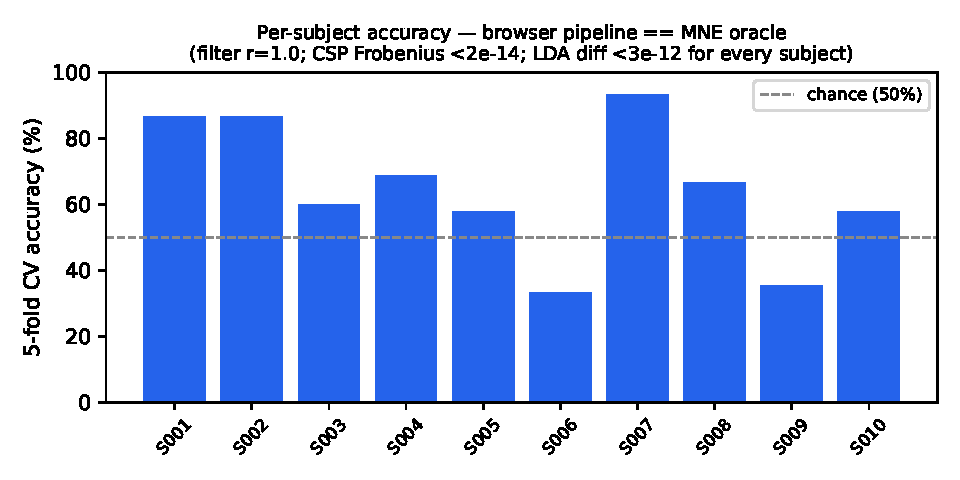
\includegraphics[width=\columnwidth]{../shared/figures/accuracy.pdf}
\caption{Per-subject \Folds-fold accuracy (S001--S010); browser equals MNE oracle to machine
precision for every subject.}\label{fig:acc}\end{figure}

\begin{figure}[!t]\centering
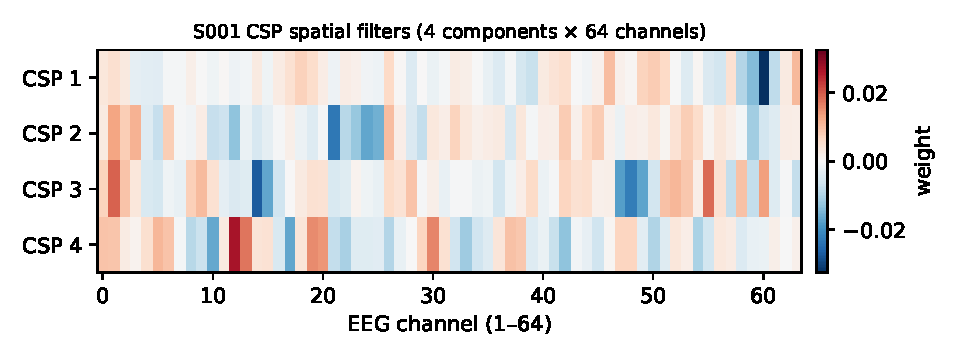
\includegraphics[width=\columnwidth]{../shared/figures/csp_s001.pdf}
\caption{S001 CSP spatial filters (\CspComp{} components $\times$ \Nchannels{} channels).}
\label{fig:csp}\end{figure}

\subsection{Performance}
A Playwright-driven headless-Chromium benchmark (\HwCpu{}, \HwCores{}~cores, \HwRam~GB; \HwBrowser{};
N=\Nreps{}) gives a full-pipeline runtime of \WorkerOneX$\pm$\WorkerOneXStd~ms in the Web Worker and a
peak JavaScript heap of \PeakHeap~MB (Fig.~\ref{fig:perf}). An honest measurement caveat emerged: the
browser devtools-protocol CPU throttle reaches the renderer main thread but not Web Workers, so
worker timings are essentially flat across throttle rates. We therefore measured a CPU-slowdown proxy
by running the identical computation on the throttled main thread, obtaining
\ProxyOneX{}/\ProxyFourX{}/\ProxySixX~ms at $1\times$/$4\times$/$6\times$ (Fig.~\ref{fig:throttle}).
These are a proxy; a physical low-specification device measurement remains future
work~\todo{physical low-spec device run}.

\begin{figure}[!t]\centering
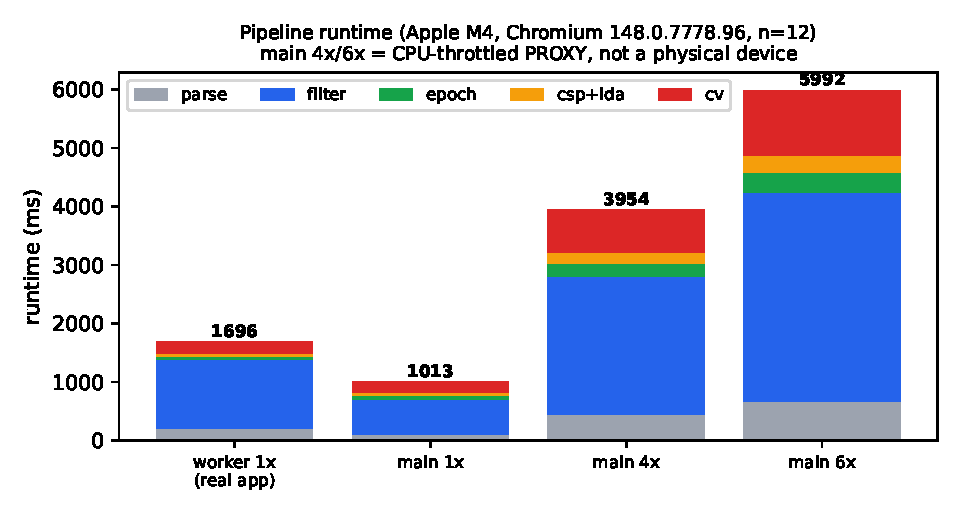
\includegraphics[width=\columnwidth]{../shared/figures/performance.pdf}
\caption{Measured runtime on real hardware: Web Worker (real app) and the identical computation on a
throttled main thread (CPU-slowdown proxy; $4\times$/$6\times$ are not a physical device).}
\label{fig:perf}\end{figure}

\begin{figure}[!t]\centering
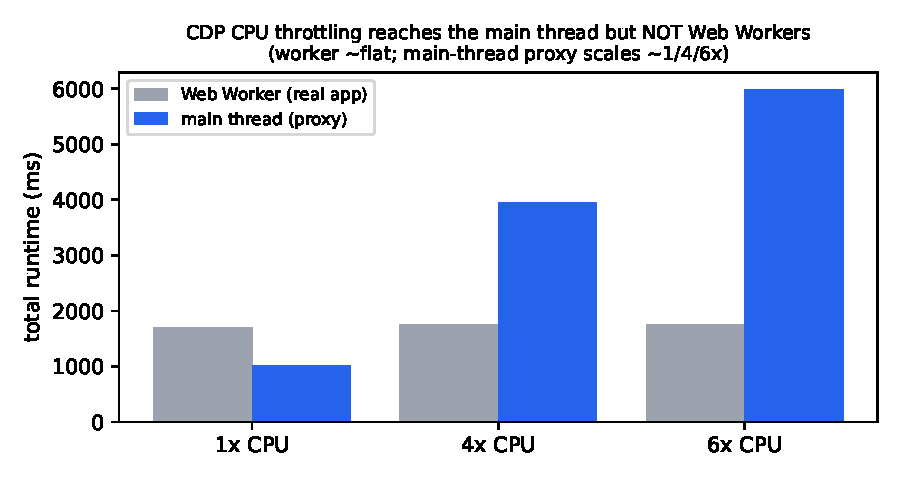
\includegraphics[width=\columnwidth]{../shared/figures/throttle_finding.pdf}
\caption{Devtools CPU throttling reaches the main thread but not Web Workers: worker timings are
flat while the main-thread proxy scales with the throttle factor.}\label{fig:throttle}\end{figure}

\section{Discussion}
By removing installation, the tool lowers the barrier to running standard EEG motor-imagery analysis:
a reader can re-run an analysis from a link, instructors avoid environment setup, and the analysis
runs on restricted or low-resource machines (an edge/accessibility angle). The validation
methodology generalizes to any port of a scientific pipeline to a new runtime. \emph{Limitations:}
the validated dataset format is EDF/EDF+ (GDF support is routed through a pre-conversion adapter and
not yet validated); the equivalence study covers \Nsubjects{} subjects of one dataset; and the
low-specification fit is argued from a \PeakHeap~MB peak heap measured on capable hardware---a
documented assumption pending a physical-device run. The contribution is reproduction and validation,
not a new decoding method.

\section{Conclusion}
We presented a fully client-side EEG motor-imagery analysis tool that reproduces an
MNE-Python/scikit-learn reference to machine precision across \Nsubjects{} subjects, with real
in-browser performance measurements and an explicit, honest account of what was and was not measured.
The work delivers a validated, reproducible, install-free artifact for EEG/BCI analysis.

\section*{Acknowledgment}
\todo{acknowledgments, if any}

\bibliographystyle{IEEEtran}
\bibliography{../shared/refs}

\vspace{6pt}
\noindent\textbf{Author biography:} \todo{Eugene Cha biography and photo}

\end{document}
